\begin{figure}
    \centering
    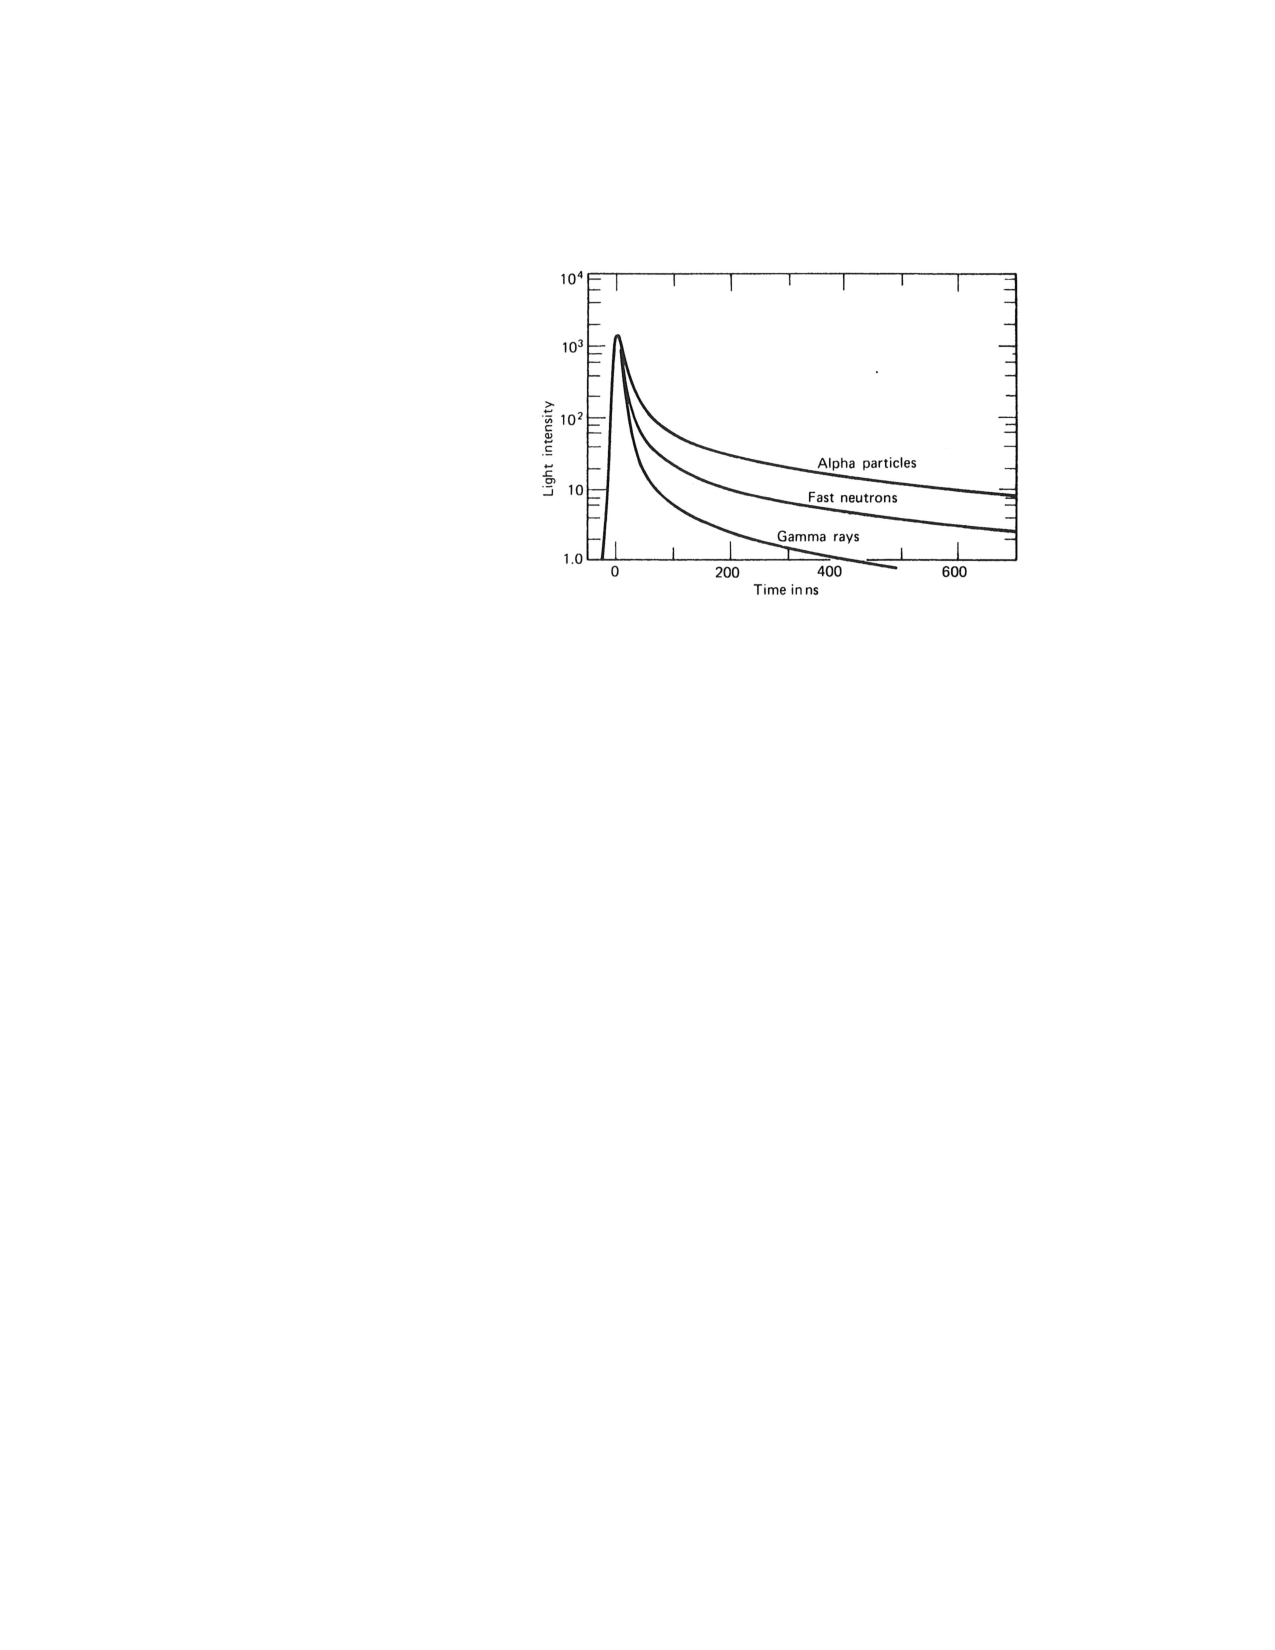
\includegraphics{Setup_Figs/pulse_shape.pdf}
    \caption{A cartoon illustration of pulse shape based on radiation type, in the same detecting material. The different types of radiation interact with the detecting material creating a fast and slow excitation. The ratio of these fast and slow excitations is based on the radiation, and expressed in the length of the decay tail. Picture taken from \citep{knoll00:rad_det_meas}.}
    \label{fig:pulse_discrimination}
\end{figure}